\documentclass[twoside]{book}

% Packages required by doxygen
\usepackage{calc}
\usepackage{doxygen}
\usepackage{graphicx}
\usepackage[utf8]{inputenc}
\usepackage{makeidx}
\usepackage{multicol}
\usepackage{multirow}
\usepackage{textcomp}
\usepackage[table]{xcolor}

% Font selection
\usepackage[T1]{fontenc}
\usepackage{mathptmx}
\usepackage[scaled=.90]{helvet}
\usepackage{courier}
\usepackage{amssymb}
\usepackage{sectsty}
\renewcommand{\familydefault}{\sfdefault}
\allsectionsfont{%
  \fontseries{bc}\selectfont%
  \color{darkgray}%
}
\renewcommand{\DoxyLabelFont}{%
  \fontseries{bc}\selectfont%
  \color{darkgray}%
}

% Page & text layout
\usepackage{geometry}
\geometry{%
  a4paper,%
  top=2.5cm,%
  bottom=2.5cm,%
  left=2.5cm,%
  right=2.5cm%
}
\tolerance=750
\hfuzz=15pt
\hbadness=750
\setlength{\emergencystretch}{15pt}
\setlength{\parindent}{0cm}
\setlength{\parskip}{0.2cm}
\makeatletter
\renewcommand{\paragraph}{%
  \@startsection{paragraph}{4}{0ex}{-1.0ex}{1.0ex}{%
    \normalfont\normalsize\bfseries\SS@parafont%
  }%
}
\renewcommand{\subparagraph}{%
  \@startsection{subparagraph}{5}{0ex}{-1.0ex}{1.0ex}{%
    \normalfont\normalsize\bfseries\SS@subparafont%
  }%
}
\makeatother

% Headers & footers
\usepackage{fancyhdr}
\pagestyle{fancyplain}
\fancyhead[LE]{\fancyplain{}{\bfseries\thepage}}
\fancyhead[CE]{\fancyplain{}{}}
\fancyhead[RE]{\fancyplain{}{\bfseries\leftmark}}
\fancyhead[LO]{\fancyplain{}{\bfseries\rightmark}}
\fancyhead[CO]{\fancyplain{}{}}
\fancyhead[RO]{\fancyplain{}{\bfseries\thepage}}
\fancyfoot[LE]{\fancyplain{}{}}
\fancyfoot[CE]{\fancyplain{}{}}
\fancyfoot[RE]{\fancyplain{}{\bfseries\scriptsize Generated on Sun Nov 15 2015 20\-:39\-:31 for Gym\-Management by Doxygen }}
\fancyfoot[LO]{\fancyplain{}{\bfseries\scriptsize Generated on Sun Nov 15 2015 20\-:39\-:31 for Gym\-Management by Doxygen }}
\fancyfoot[CO]{\fancyplain{}{}}
\fancyfoot[RO]{\fancyplain{}{}}
\renewcommand{\footrulewidth}{0.4pt}
\renewcommand{\chaptermark}[1]{%
  \markboth{#1}{}%
}
\renewcommand{\sectionmark}[1]{%
  \markright{\thesection\ #1}%
}

% Indices & bibliography
\usepackage{natbib}
\usepackage[titles]{tocloft}
\setcounter{tocdepth}{3}
\setcounter{secnumdepth}{5}
\makeindex

% Hyperlinks (required, but should be loaded last)
\usepackage{ifpdf}
\ifpdf
  \usepackage[pdftex,pagebackref=true]{hyperref}
\else
  \usepackage[ps2pdf,pagebackref=true]{hyperref}
\fi
\hypersetup{%
  colorlinks=true,%
  linkcolor=blue,%
  citecolor=blue,%
  unicode%
}

% Custom commands
\newcommand{\clearemptydoublepage}{%
  \newpage{\pagestyle{empty}\cleardoublepage}%
}


%===== C O N T E N T S =====

\begin{document}

% Titlepage & ToC
\hypersetup{pageanchor=false}
\pagenumbering{roman}
\begin{titlepage}
\vspace*{7cm}
\begin{center}%
{\Large Gym\-Management }\\
\vspace*{1cm}
{\large Generated by Doxygen 1.8.6}\\
\vspace*{0.5cm}
{\small Sun Nov 15 2015 20:39:31}\\
\end{center}
\end{titlepage}
\clearemptydoublepage
\tableofcontents
\clearemptydoublepage
\pagenumbering{arabic}
\hypersetup{pageanchor=true}

%--- Begin generated contents ---
\chapter{Hierarchical Index}
\section{Class Hierarchy}
This inheritance list is sorted roughly, but not completely, alphabetically\-:\begin{DoxyCompactList}
\item \contentsline{section}{Activity\-Profile}{\pageref{class_activity_profile}}{}
\item \contentsline{section}{Equipment}{\pageref{class_equipment}}{}
\item \contentsline{section}{Fitness\-Lesson}{\pageref{class_fitness_lesson}}{}
\item \contentsline{section}{Membership\-Controller}{\pageref{class_membership_controller}}{}
\item \contentsline{section}{Member\-View}{\pageref{class_member_view}}{}
\item \contentsline{section}{Person}{\pageref{class_person}}{}
\begin{DoxyCompactList}
\item \contentsline{section}{Employee}{\pageref{class_employee}}{}
\item \contentsline{section}{Member}{\pageref{class_member}}{}
\end{DoxyCompactList}
\item \contentsline{section}{Schedule\-Controller}{\pageref{class_schedule_controller}}{}
\item \contentsline{section}{Workout\-Plan}{\pageref{class_workout_plan}}{}
\end{DoxyCompactList}

\chapter{Class Index}
\section{Class List}
Here are the classes, structs, unions and interfaces with brief descriptions\-:\begin{DoxyCompactList}
\item\contentsline{section}{\hyperlink{class_activity_profile}{Activity\-Profile} }{\pageref{class_activity_profile}}{}
\item\contentsline{section}{\hyperlink{class_employee}{Employee} }{\pageref{class_employee}}{}
\item\contentsline{section}{\hyperlink{class_equipment}{Equipment} }{\pageref{class_equipment}}{}
\item\contentsline{section}{\hyperlink{class_fitness_lesson}{Fitness\-Lesson} }{\pageref{class_fitness_lesson}}{}
\item\contentsline{section}{\hyperlink{class_member}{Member} }{\pageref{class_member}}{}
\item\contentsline{section}{\hyperlink{class_membership_controller}{Membership\-Controller} }{\pageref{class_membership_controller}}{}
\item\contentsline{section}{\hyperlink{class_member_view}{Member\-View} }{\pageref{class_member_view}}{}
\item\contentsline{section}{\hyperlink{class_person}{Person} }{\pageref{class_person}}{}
\item\contentsline{section}{\hyperlink{class_schedule_controller}{Schedule\-Controller} }{\pageref{class_schedule_controller}}{}
\item\contentsline{section}{\hyperlink{class_workout_plan}{Workout\-Plan} }{\pageref{class_workout_plan}}{}
\end{DoxyCompactList}

\chapter{Class Documentation}
\hypertarget{class_activity_profile}{\section{Activity\-Profile Class Reference}
\label{class_activity_profile}\index{Activity\-Profile@{Activity\-Profile}}
}
\subsection*{Public Member Functions}
\begin{DoxyCompactItemize}
\item 
void \hyperlink{class_activity_profile_aedc076416b2f4dbb39bb3a7566b7daee}{Calculate\-Trends} ()
\end{DoxyCompactItemize}
\subsection*{Public Attributes}
\begin{DoxyCompactItemize}
\item 
\hypertarget{class_activity_profile_af74beabb58b683e3e247c406cece3d7d}{int {\bfseries stats}}\label{class_activity_profile_af74beabb58b683e3e247c406cece3d7d}

\end{DoxyCompactItemize}


\subsection{Member Function Documentation}
\hypertarget{class_activity_profile_aedc076416b2f4dbb39bb3a7566b7daee}{\index{Activity\-Profile@{Activity\-Profile}!Calculate\-Trends@{Calculate\-Trends}}
\index{Calculate\-Trends@{Calculate\-Trends}!ActivityProfile@{Activity\-Profile}}
\subsubsection[{Calculate\-Trends}]{\setlength{\rightskip}{0pt plus 5cm}void Activity\-Profile\-::\-Calculate\-Trends (
\begin{DoxyParamCaption}
{}
\end{DoxyParamCaption}
)}}\label{class_activity_profile_aedc076416b2f4dbb39bb3a7566b7daee}
Outputs meaningful statistics about the users activity profile 

The documentation for this class was generated from the following files\-:\begin{DoxyCompactItemize}
\item 
activityprofile.\-h\item 
activityprofile.\-cpp\end{DoxyCompactItemize}

\hypertarget{class_employee}{\section{Employee Class Reference}
\label{class_employee}\index{Employee@{Employee}}
}
Inheritance diagram for Employee\-:\begin{figure}[H]
\begin{center}
\leavevmode
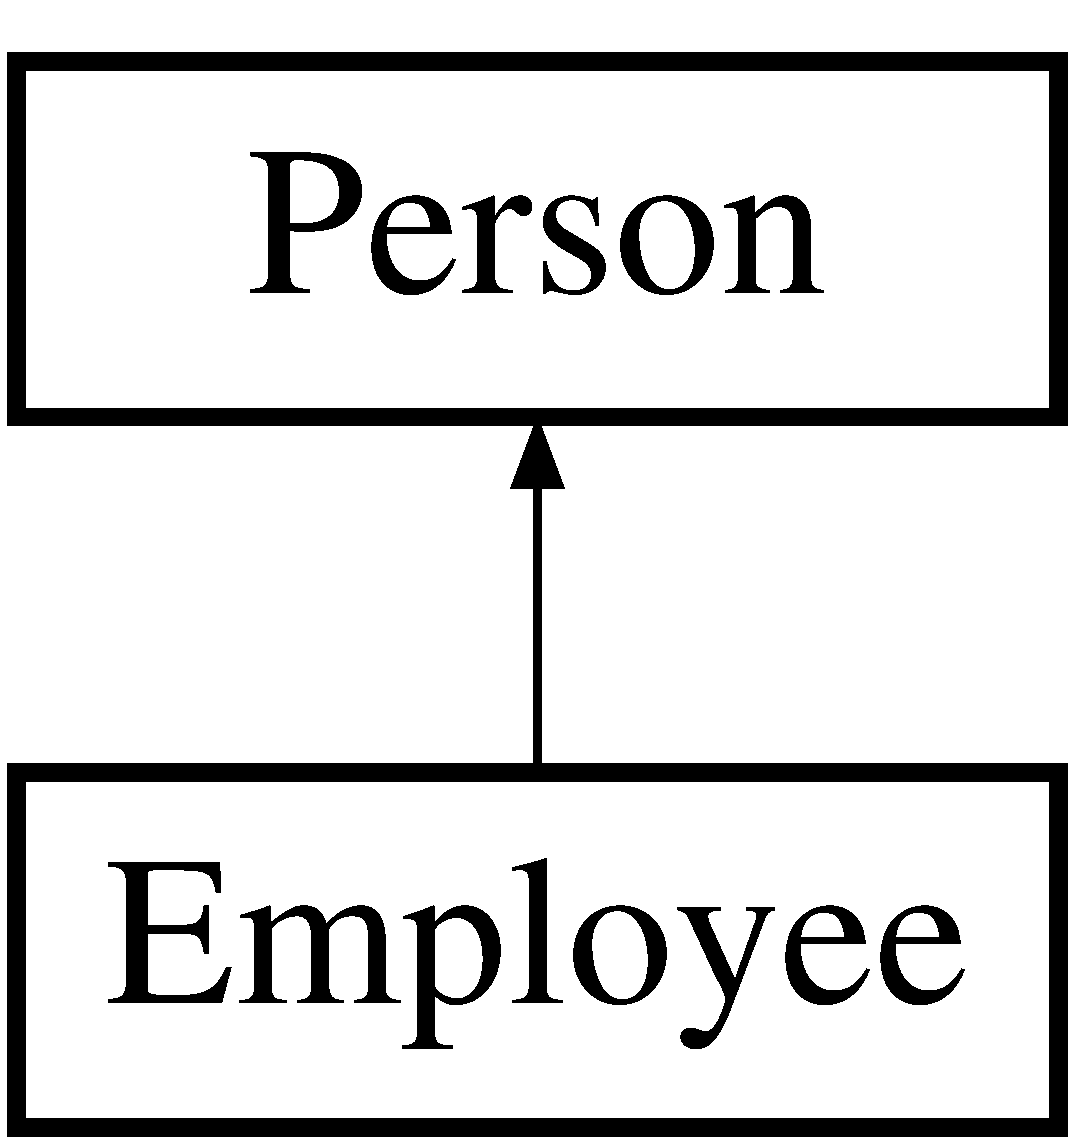
\includegraphics[height=2.000000cm]{class_employee}
\end{center}
\end{figure}
\subsection*{Public Member Functions}
\begin{DoxyCompactItemize}
\item 
virtual \hyperlink{class_person}{Person} $\ast$ \hyperlink{class_employee_ad5b1f55ab3c2aea17306fc360f3abe78}{clone} ()
\end{DoxyCompactItemize}
\subsection*{Public Attributes}
\begin{DoxyCompactItemize}
\item 
\hypertarget{class_employee_a4169fe4ef43dbc0bb14e5fff53b2a435}{int {\bfseries hours\-Per\-Week}}\label{class_employee_a4169fe4ef43dbc0bb14e5fff53b2a435}

\end{DoxyCompactItemize}


\subsection{Member Function Documentation}
\hypertarget{class_employee_ad5b1f55ab3c2aea17306fc360f3abe78}{\index{Employee@{Employee}!clone@{clone}}
\index{clone@{clone}!Employee@{Employee}}
\subsubsection[{clone}]{\setlength{\rightskip}{0pt plus 5cm}{\bf Person} $\ast$ Employee\-::clone (
\begin{DoxyParamCaption}
{}
\end{DoxyParamCaption}
)\hspace{0.3cm}{\ttfamily [virtual]}}}\label{class_employee_ad5b1f55ab3c2aea17306fc360f3abe78}
Clones the current isntance 

Implements \hyperlink{class_person}{Person}.



The documentation for this class was generated from the following files\-:\begin{DoxyCompactItemize}
\item 
employee.\-h\item 
employee.\-cpp\end{DoxyCompactItemize}

\hypertarget{class_equipment}{\section{Equipment Class Reference}
\label{class_equipment}\index{Equipment@{Equipment}}
}
\subsection*{Public Attributes}
\begin{DoxyCompactItemize}
\item 
\hypertarget{class_equipment_a77c1240ba821ee049a9834e06f2b52a9}{int {\bfseries id}}\label{class_equipment_a77c1240ba821ee049a9834e06f2b52a9}

\end{DoxyCompactItemize}


The documentation for this class was generated from the following files\-:\begin{DoxyCompactItemize}
\item 
equipment.\-h\item 
equipment.\-cpp\end{DoxyCompactItemize}

\hypertarget{class_fitness_lesson}{\section{Fitness\-Lesson Class Reference}
\label{class_fitness_lesson}\index{Fitness\-Lesson@{Fitness\-Lesson}}
}
\subsection*{Public Attributes}
\begin{DoxyCompactItemize}
\item 
\hypertarget{class_fitness_lesson_ad70e19a363a1cec4bfbf84ddb0269c98}{time\-\_\-t {\bfseries time}}\label{class_fitness_lesson_ad70e19a363a1cec4bfbf84ddb0269c98}

\item 
\hypertarget{class_fitness_lesson_a5dd91cc4512335304ff67e5fff54099e}{int {\bfseries duration}}\label{class_fitness_lesson_a5dd91cc4512335304ff67e5fff54099e}

\item 
\hypertarget{class_fitness_lesson_a25c4e6328a305fda4f39f19edf70238c}{\hyperlink{class_employee}{Employee} {\bfseries instructor}}\label{class_fitness_lesson_a25c4e6328a305fda4f39f19edf70238c}

\end{DoxyCompactItemize}


The documentation for this class was generated from the following files\-:\begin{DoxyCompactItemize}
\item 
fitnesslesson.\-h\item 
fitnesslesson.\-cpp\end{DoxyCompactItemize}

\hypertarget{class_member}{\section{Member Class Reference}
\label{class_member}\index{Member@{Member}}
}
Inheritance diagram for Member\-:\begin{figure}[H]
\begin{center}
\leavevmode
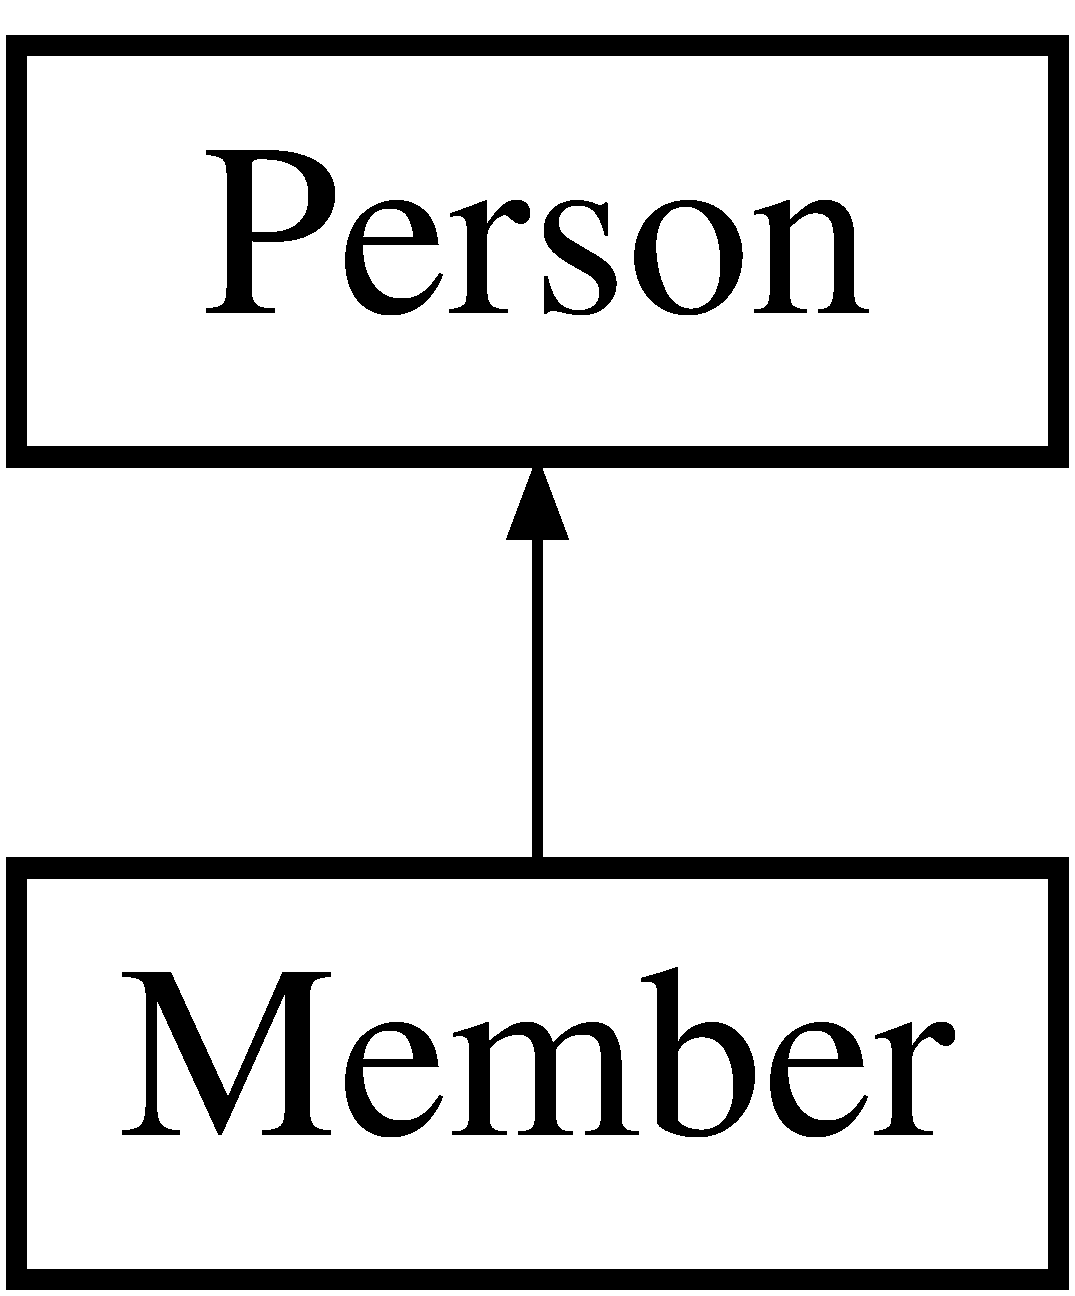
\includegraphics[height=2.000000cm]{class_member}
\end{center}
\end{figure}
\subsection*{Public Member Functions}
\begin{DoxyCompactItemize}
\item 
void \hyperlink{class_member_ac5f0fc7e6f535f3de006aee2c90055d8}{add\-Class} (\hyperlink{class_fitness_lesson}{Fitness\-Lesson} l)
\item 
\hypertarget{class_member_afed2e992a20ebe55afc1272bdbdba6ac}{virtual \hyperlink{class_person}{Person} $\ast$ {\bfseries clone} ()}\label{class_member_afed2e992a20ebe55afc1272bdbdba6ac}

\end{DoxyCompactItemize}
\subsection*{Public Attributes}
\begin{DoxyCompactItemize}
\item 
\hypertarget{class_member_a3066542e3f1e6a96c832c7fc9fa94079}{int {\bfseries activity\-Level}}\label{class_member_a3066542e3f1e6a96c832c7fc9fa94079}

\end{DoxyCompactItemize}


\subsection{Member Function Documentation}
\hypertarget{class_member_ac5f0fc7e6f535f3de006aee2c90055d8}{\index{Member@{Member}!add\-Class@{add\-Class}}
\index{add\-Class@{add\-Class}!Member@{Member}}
\subsubsection[{add\-Class}]{\setlength{\rightskip}{0pt plus 5cm}void Member\-::add\-Class (
\begin{DoxyParamCaption}
\item[{{\bf Fitness\-Lesson}}]{l}
\end{DoxyParamCaption}
)}}\label{class_member_ac5f0fc7e6f535f3de006aee2c90055d8}
Adds a class to the member's workout plan 

The documentation for this class was generated from the following files\-:\begin{DoxyCompactItemize}
\item 
member.\-h\item 
member.\-cpp\end{DoxyCompactItemize}

\hypertarget{class_membership_controller}{\section{Membership\-Controller Class Reference}
\label{class_membership_controller}\index{Membership\-Controller@{Membership\-Controller}}
}


{\ttfamily \#include $<$membershipcontroller.\-h$>$}

\subsection*{Public Member Functions}
\begin{DoxyCompactItemize}
\item 
void \hyperlink{class_membership_controller_a5dee58ec4865052d85156b9f042b429c}{add\-Member} (\hyperlink{class_member}{Member} m)
\item 
void \hyperlink{class_membership_controller_acfdd3d9ccaa56cf6f41c4237c2d47f14}{check\-Membership\-Expiry} (\hyperlink{class_member}{Member} m)
\item 
void \hyperlink{class_membership_controller_af26d202b3274cfff1d2bb8cb2b2f0784}{delete\-Member} (\hyperlink{class_member}{Member} m)
\item 
\hyperlink{class_activity_profile}{Activity\-Profile} \hyperlink{class_membership_controller_a15765068736138fadf8837a7a7a05ad2}{get\-Member\-Activity\-Profile} (\hyperlink{class_member}{Member} m)
\end{DoxyCompactItemize}
\subsection*{Public Attributes}
\begin{DoxyCompactItemize}
\item 
std\-::vector$<$ \hyperlink{class_person}{Person} $\ast$ $>$ \hyperlink{class_membership_controller_ab1ba5783f942d4df197a6d6b35ff40ee}{person\-List}
\end{DoxyCompactItemize}


\subsection{Detailed Description}
Controlls the status of all the members 

\subsection{Member Function Documentation}
\hypertarget{class_membership_controller_a5dee58ec4865052d85156b9f042b429c}{\index{Membership\-Controller@{Membership\-Controller}!add\-Member@{add\-Member}}
\index{add\-Member@{add\-Member}!MembershipController@{Membership\-Controller}}
\subsubsection[{add\-Member}]{\setlength{\rightskip}{0pt plus 5cm}void Membership\-Controller\-::add\-Member (
\begin{DoxyParamCaption}
\item[{{\bf Member}}]{m}
\end{DoxyParamCaption}
)}}\label{class_membership_controller_a5dee58ec4865052d85156b9f042b429c}
Adds a member to the database 
\begin{DoxyParams}{Parameters}
{\em \hyperlink{class_member}{Member}} & m -\/ The member to be added \\
\hline
\end{DoxyParams}
\hypertarget{class_membership_controller_acfdd3d9ccaa56cf6f41c4237c2d47f14}{\index{Membership\-Controller@{Membership\-Controller}!check\-Membership\-Expiry@{check\-Membership\-Expiry}}
\index{check\-Membership\-Expiry@{check\-Membership\-Expiry}!MembershipController@{Membership\-Controller}}
\subsubsection[{check\-Membership\-Expiry}]{\setlength{\rightskip}{0pt plus 5cm}void Membership\-Controller\-::check\-Membership\-Expiry (
\begin{DoxyParamCaption}
\item[{{\bf Member}}]{m}
\end{DoxyParamCaption}
)}}\label{class_membership_controller_acfdd3d9ccaa56cf6f41c4237c2d47f14}
Checks a member's expiry 
\begin{DoxyParams}{Parameters}
{\em \hyperlink{class_member}{Member}} & m -\/ The membership to be investigated \\
\hline
\end{DoxyParams}
\hypertarget{class_membership_controller_af26d202b3274cfff1d2bb8cb2b2f0784}{\index{Membership\-Controller@{Membership\-Controller}!delete\-Member@{delete\-Member}}
\index{delete\-Member@{delete\-Member}!MembershipController@{Membership\-Controller}}
\subsubsection[{delete\-Member}]{\setlength{\rightskip}{0pt plus 5cm}void Membership\-Controller\-::delete\-Member (
\begin{DoxyParamCaption}
\item[{{\bf Member}}]{m}
\end{DoxyParamCaption}
)}}\label{class_membership_controller_af26d202b3274cfff1d2bb8cb2b2f0784}
Deletes a member from the database 
\begin{DoxyParams}{Parameters}
{\em \hyperlink{class_member}{Member}} & m -\/ The member to be deleted \\
\hline
\end{DoxyParams}
\hypertarget{class_membership_controller_a15765068736138fadf8837a7a7a05ad2}{\index{Membership\-Controller@{Membership\-Controller}!get\-Member\-Activity\-Profile@{get\-Member\-Activity\-Profile}}
\index{get\-Member\-Activity\-Profile@{get\-Member\-Activity\-Profile}!MembershipController@{Membership\-Controller}}
\subsubsection[{get\-Member\-Activity\-Profile}]{\setlength{\rightskip}{0pt plus 5cm}{\bf Activity\-Profile} Membership\-Controller\-::get\-Member\-Activity\-Profile (
\begin{DoxyParamCaption}
\item[{{\bf Member}}]{m}
\end{DoxyParamCaption}
)}}\label{class_membership_controller_a15765068736138fadf8837a7a7a05ad2}
Returns the members activity profile with enhanced statistics 
\begin{DoxyParams}{Parameters}
{\em \hyperlink{class_member}{Member}} & m -\/ The member whose profile is desired \\
\hline
\end{DoxyParams}
\begin{DoxyReturn}{Returns}
\hyperlink{class_activity_profile}{Activity\-Profile} -\/ The activity of  m 
\end{DoxyReturn}


\subsection{Member Data Documentation}
\hypertarget{class_membership_controller_ab1ba5783f942d4df197a6d6b35ff40ee}{\index{Membership\-Controller@{Membership\-Controller}!person\-List@{person\-List}}
\index{person\-List@{person\-List}!MembershipController@{Membership\-Controller}}
\subsubsection[{person\-List}]{\setlength{\rightskip}{0pt plus 5cm}std\-::vector$<${\bf Person}$\ast$$>$ Membership\-Controller\-::person\-List}}\label{class_membership_controller_ab1ba5783f942d4df197a6d6b35ff40ee}
The list of current members and employees 

The documentation for this class was generated from the following files\-:\begin{DoxyCompactItemize}
\item 
membershipcontroller.\-h\item 
membershipcontroller.\-cpp\end{DoxyCompactItemize}

\hypertarget{class_member_view}{\section{Member\-View Class Reference}
\label{class_member_view}\index{Member\-View@{Member\-View}}
}
\subsection*{Public Member Functions}
\begin{DoxyCompactItemize}
\item 
\hypertarget{class_member_view_a4fc868363bf3c76ef7cf236d562e3ca8}{void {\bfseries view\-Workout\-Plan} (\hyperlink{class_member}{Member} m)}\label{class_member_view_a4fc868363bf3c76ef7cf236d562e3ca8}

\item 
\hypertarget{class_member_view_acc39fce53b81172f8c96e03c712405d3}{void {\bfseries view\-Class\-List} ()}\label{class_member_view_acc39fce53b81172f8c96e03c712405d3}

\item 
\hypertarget{class_member_view_a8f52d402f1df0b37afa7408e2c706bf5}{void {\bfseries reserve\-Trainer} (\hyperlink{class_employee}{Employee} e)}\label{class_member_view_a8f52d402f1df0b37afa7408e2c706bf5}

\item 
\hypertarget{class_member_view_a75164319c4ca544ab3b23bcbf7bfbc62}{void {\bfseries insert\-Class} (\hyperlink{class_fitness_lesson}{Fitness\-Lesson} l)}\label{class_member_view_a75164319c4ca544ab3b23bcbf7bfbc62}

\item 
\hypertarget{class_member_view_a866da036d8cd19b44da086f703150dd3}{void {\bfseries make\-Payment} ()}\label{class_member_view_a866da036d8cd19b44da086f703150dd3}

\item 
\hypertarget{class_member_view_ad9b2d42dfbec0ac20558bf2b5ad88d0e}{void {\bfseries vew\-Activity\-Profile} (\hyperlink{class_member}{Member} m)}\label{class_member_view_ad9b2d42dfbec0ac20558bf2b5ad88d0e}

\end{DoxyCompactItemize}


The documentation for this class was generated from the following files\-:\begin{DoxyCompactItemize}
\item 
memberview.\-h\item 
memberview.\-cpp\end{DoxyCompactItemize}

\hypertarget{class_person}{\section{Person Class Reference}
\label{class_person}\index{Person@{Person}}
}
Inheritance diagram for Person\-:\begin{figure}[H]
\begin{center}
\leavevmode
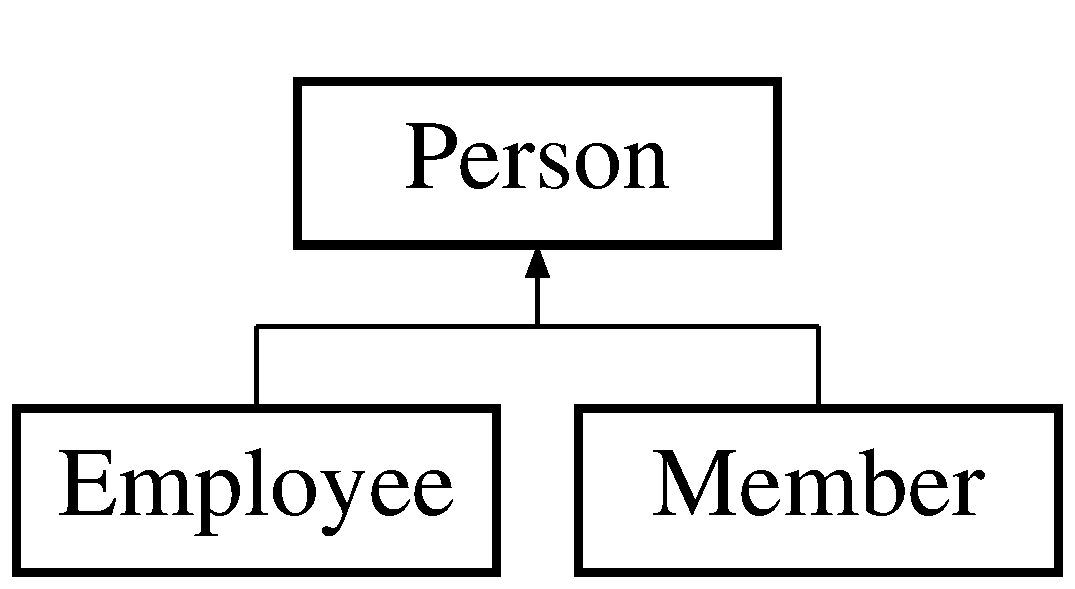
\includegraphics[height=2.000000cm]{class_person}
\end{center}
\end{figure}
\subsection*{Public Member Functions}
\begin{DoxyCompactItemize}
\item 
\hypertarget{class_person_a1b1099a7fe99bd551e8785d7458a560f}{virtual \hyperlink{class_person}{Person} $\ast$ {\bfseries clone} ()=0}\label{class_person_a1b1099a7fe99bd551e8785d7458a560f}

\end{DoxyCompactItemize}
\subsection*{Public Attributes}
\begin{DoxyCompactItemize}
\item 
\hypertarget{class_person_a7594663aadc0de77616506df8a2f4128}{std\-::string {\bfseries name}}\label{class_person_a7594663aadc0de77616506df8a2f4128}

\item 
\hypertarget{class_person_aec48a92f614a854ff380a15eb8e2f479}{int {\bfseries id}}\label{class_person_aec48a92f614a854ff380a15eb8e2f479}

\end{DoxyCompactItemize}


The documentation for this class was generated from the following files\-:\begin{DoxyCompactItemize}
\item 
person.\-h\item 
person.\-cpp\end{DoxyCompactItemize}

\hypertarget{class_schedule_controller}{\section{Schedule\-Controller Class Reference}
\label{class_schedule_controller}\index{Schedule\-Controller@{Schedule\-Controller}}
}
\subsection*{Public Member Functions}
\begin{DoxyCompactItemize}
\item 
\hypertarget{class_schedule_controller_a3c8ff579f30865270072b43043047f88}{void {\bfseries create\-Class} (\hyperlink{class_fitness_lesson}{Fitness\-Lesson} l)}\label{class_schedule_controller_a3c8ff579f30865270072b43043047f88}

\item 
\hypertarget{class_schedule_controller_ae12d0dbcfc66e3b40938284237376c0d}{void {\bfseries get\-Class\-List} ()}\label{class_schedule_controller_ae12d0dbcfc66e3b40938284237376c0d}

\end{DoxyCompactItemize}


The documentation for this class was generated from the following files\-:\begin{DoxyCompactItemize}
\item 
schedulecontroller.\-h\item 
schedulecontroller.\-cpp\end{DoxyCompactItemize}

\hypertarget{class_workout_plan}{\section{Workout\-Plan Class Reference}
\label{class_workout_plan}\index{Workout\-Plan@{Workout\-Plan}}
}
\subsection*{Public Member Functions}
\begin{DoxyCompactItemize}
\item 
\hypertarget{class_workout_plan_a634f7753ebe7a07a31ef07da04733a7b}{void {\bfseries generate\-Workout} ()}\label{class_workout_plan_a634f7753ebe7a07a31ef07da04733a7b}

\end{DoxyCompactItemize}


The documentation for this class was generated from the following files\-:\begin{DoxyCompactItemize}
\item 
workoutplan.\-h\item 
workoutplan.\-cpp\end{DoxyCompactItemize}

%--- End generated contents ---

% Index
\newpage
\phantomsection
\addcontentsline{toc}{chapter}{Index}
\printindex

\end{document}
